\item For the given matrix $$\vec{Q}=\myvec{\frac{1}{\sqrt{2}}&0&\frac{1}{\sqrt{2}}\\
0&1&0\\
-\frac{1}{\sqrt{2}}&0&\frac{1}{\sqrt{2}}},$$ which of the following statements is/are true?
\hfill{(PE 2024)}
\begin{enumerate}
	\begin{multicols}{2}
    \item $\vec{Q}$ is an orthogonal matrix
    \item $\vec{Q}^{\top}=\vec{Q}^{-1}$
    \item $\vec{Q}$ is a singular matrix
    \item $\vec{Q}$ is a symmetric matrix
    \end{multicols}
\end{enumerate}
\item If $\vec{P}=\myvec{2&-1\\
2&2}$, the product of the eigenvalues of $\vec{P}$ is \dots
\hfill{(PE 2024)}
%
\item If a weight of $\vec{P}=100N$ is supported by two massless strings connected to the walls as shown in the figure, the value of $\vec{T}_1$ is \dots N.
\hfill{(PE 2024)}
\begin{figure}[H]
    \centering
    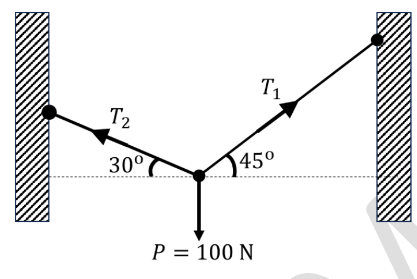
\includegraphics[width=0.5\columnwidth]{GATE/2025/PE/figs/LQ_53.png}
    \caption{}
    \label{fig:placeholder/2025/pe}
\end{figure}

